\documentclass[12pt, a4paper]{report}

\usepackage[left=1.5in, right=1in, top=1.5in, bottom=1in]{geometry}

\usepackage{titlesec}
\usepackage{natbib} % Hrvrd ref.
\usepackage[hidelinks]{hyperref}
\usepackage{makeidx} 
\usepackage{adjustbox}
\usepackage{graphicx} % Required for inserting images
\usepackage{float}    % Required for the [H] (strict "Here") positioning specifier
\makeindex

\begin{document}

\pagenumbering{roman}

\begin{titlepage}
    \centering
    \vspace*{2cm}
    \Huge\textbf{A Better Open Area}\\
    \vspace{0.5cm}
    \Large How the UCSC Open Area is used for academic and
non-academic activities across different times of the day,
and what factors influence students to choose the space
for studying versus social interaction.\\
    \vspace{6.5cm}
    \textbf{Group 08}\\
    K.B Jayawardhana - 2023/CS/078\\
    D.M.U.P Dissanayake - 2023/CS/038\\
    T Venugoban - 2023/CS/209\\
    \vspace{2cm}
    \Large \textbf{Data Summary \& Preliminary Findings (D3)}\\
    \vspace{2cm}
    SCS 3312 Research Methods\\
    \vspace{0.25cm}
    \small University of Colombo School of Computing\\
    \vfill
\end{titlepage}

\chapter*{Acknowledgment}
\addcontentsline{toc}{chapter}{Acknowledgment}
We are thankful to the students of the University of Colombo School of Computing for participating in this study. Their valuable inputs helped validate 
the findings obtained from the observations and surveys made during the research study.

We would like to thank the module coordinator of the module SCS 3312, Research Methods for all his support throughout the research process and our group members for their collaboration during the field work.

\chapter*{Abstract}
This report highlights the data summary and initial findings of the data obtained during the quantitative research phase to determine the use of the UCSC Open Area by the students for both academic and non-academic activities. The study is intended to identify the factors that affect the choice of students using the area for academic purposes. A total number of 133 respondents participated in the surveys conducted between 10 July 2026 and 14 July 2026.

The survey was developed based on the results obtained from the qualitative research conducted in the previous phase and consisted of demographic information, behavior, and environment questions related to the reason why students chose the open area to conduct their academic work. Descriptive analysis techniques were used to analyze the data obtained.

These findings show how the students use the Open Area and the key factors that affect the experience of the students. The findings reveal the most common patterns of using the Open Area by the students as well as their attitudes towards environmental conditions and facilities present in the area. The preliminary findings can also be used to verify some of the themes that were uncovered through qualitative analysis.
On the whole, the quantitative findings give the broader picture about the behavior of the students in the UCSC Open Area.
\addcontentsline{toc}{chapter}{Abstract}



% --- TOC ---
\tableofcontents
\clearpage


% --- LOF ---
\listoffigures
\addcontentsline{toc}{chapter}{List of Figures}
\clearpage

\chapter*{List of Acronyms}
\addcontentsline{toc}{chapter}{List of Acronyms}
\begin{itemize}
    \item \textbf{UCSC:} University of Colombo School of Computing
\end{itemize}
\clearpage

% --- Main Body  ---
\pagenumbering{arabic}

\chapter{Introduction}

\section{Overview of Quantitative Fieldwork}

In this part of the study, the aim was to collect data quantitatively and thus get a clearer picture of how students use the UCSC Open Area and what variables impact their choice of the area. Based on the results of the first phase of the study (D1), the quantitative field work was planned in order to collect data quantitatively and analyze the data statistically.

In order to cover changes in student usage at different times of the day, the data were collected at different hours of the day in the weekdays. All three group members took part in field work and collected the data in the following observation hours:

\begin{itemize}
    \item Morning Block (07:00 -- 11:00)
    \item Midday Block (11:00 -- 13:00)
    \item Afternoon Block (13:00 -- 16:00)
    \item Evening Block (16:00 -- 19:00)
\end{itemize}

In every observation period, two different techniques were applied in collecting quantitative data. First, a questionnaire using Google Forms was administered among students using the Open Area for data collection. In addition, an observation checklist was also applied for the collection of headcounts, activities occurring, and the environment such as weather, noise, occupancy, and lighting. The application of both methods provided a chance for comparing the reports from the respondents with the observations done in the field.
\vspace{5cm}
\section{Data Collection Summary}

The quantitative survey was carried out through Google Forms within the period of \textbf{July 10, 2026 to July 14, 2026}, consisting of three weekdays. On the other hand, eleven (11) structured observation tasks were performed within several blocks of time in order to study changes in usage of the Open Area during a day.

Originally, a total number of $N_{\text{raw}} = 140$ survey answers have been obtained. After analyzing the data set and filtering out the answers that were incorrect or incomplete, the final data set contained $N = 133$ answers.

\chapter{Findings}
Applying descriptive statistical knowledge the following findings were made.

\section{Users of the space and their usage}
\begin{figure}[H] 
    \centering
    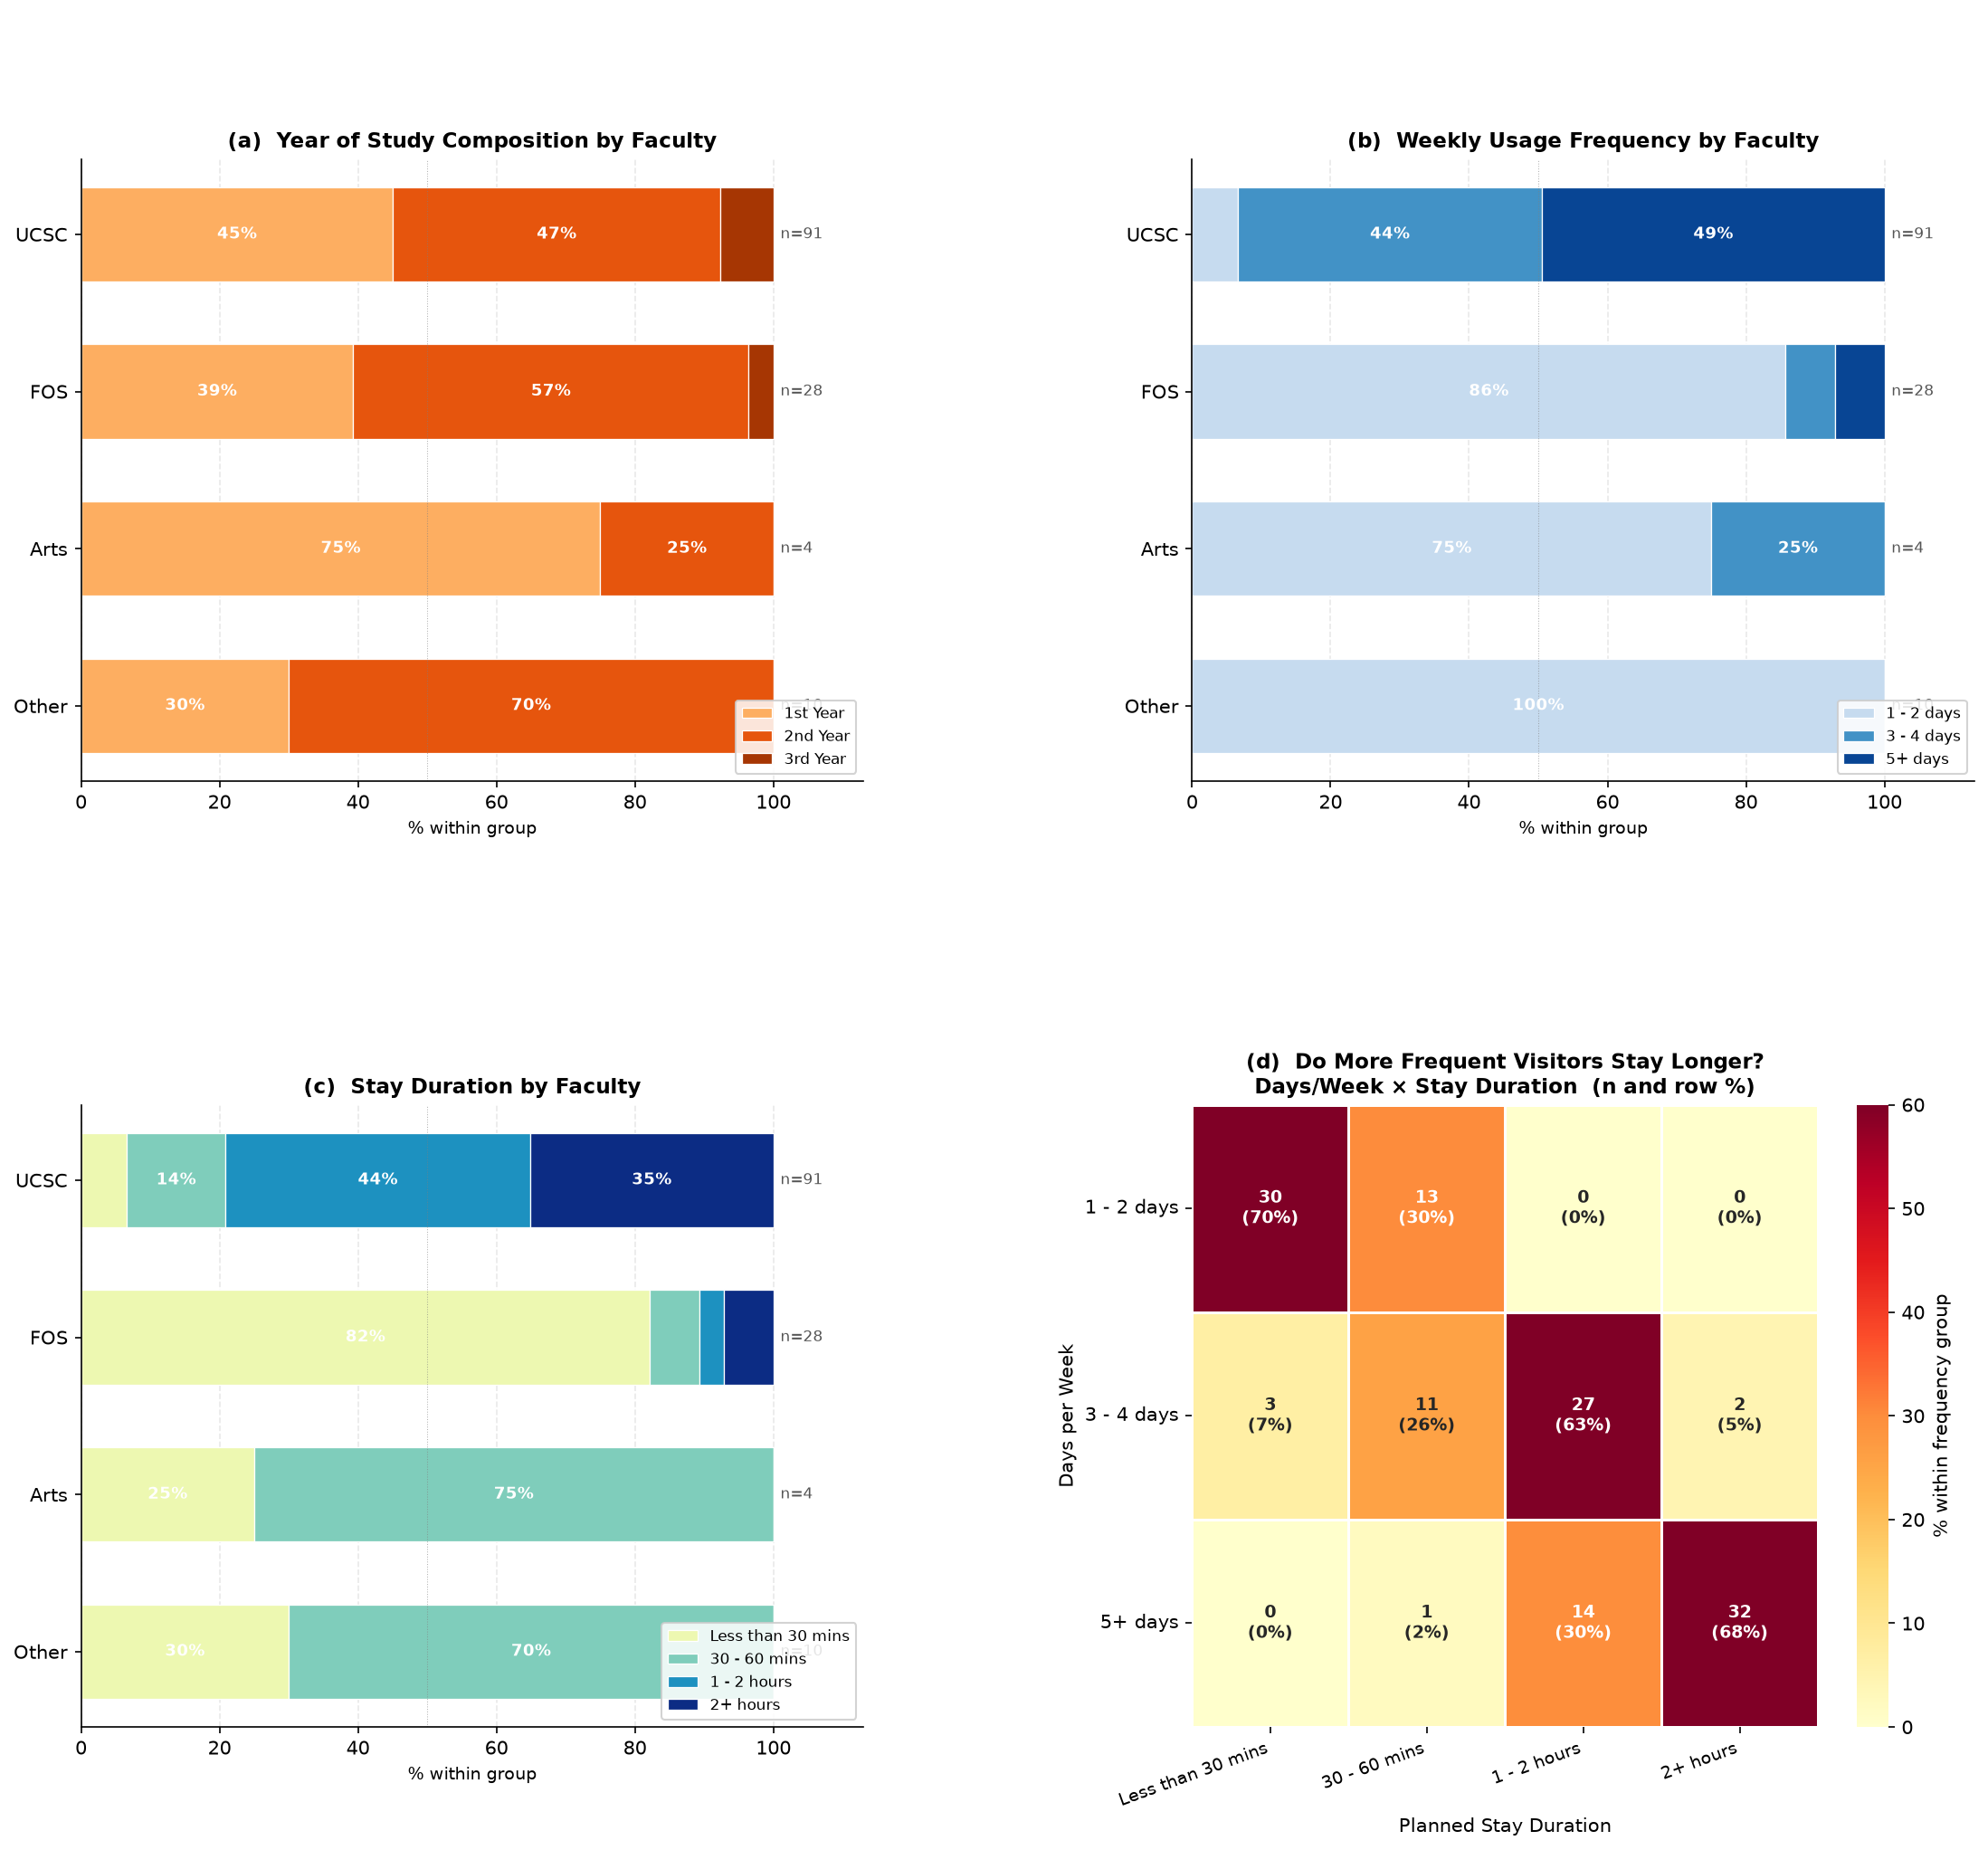
\includegraphics[width=0.7\linewidth]{descriptive_combined.png}
    \caption{Relationship between faculty, year of study, usage frequency and stay duration}
    \label{fig:demographics}
\end{figure}
The analysis of the responses from the survey participants (n = 133) shows that the Open Area is mostly used by the UCSC students (68.4\%), followed by the FOS students (21.1\%). Students from the Arts and other faculties make up a small percentage of the respondents. It can be concluded that most respondents belong to the first- and second-year students (94.0\%), meaning that the facility serves mainly younger undergraduates. Different faculty members demonstrate different use of the facility: almost half of the UCSC students visit the Open Area at least five times a week, and 79\% spend at least an hour there, which means that the facility is used regularly. In contrast, 86\% of the FOS students visit the Open Area once or twice a week, spending less than 30 minutes there (82\%). Moreover, the time spent in the area is positively correlated with the frequency of visits. Consequently, the analysis revealed that the main users of the Open Area are the first- and second-year students of the UCSC.
\section{Activities and their frequencies}
\begin{figure}[H] 
    \centering
    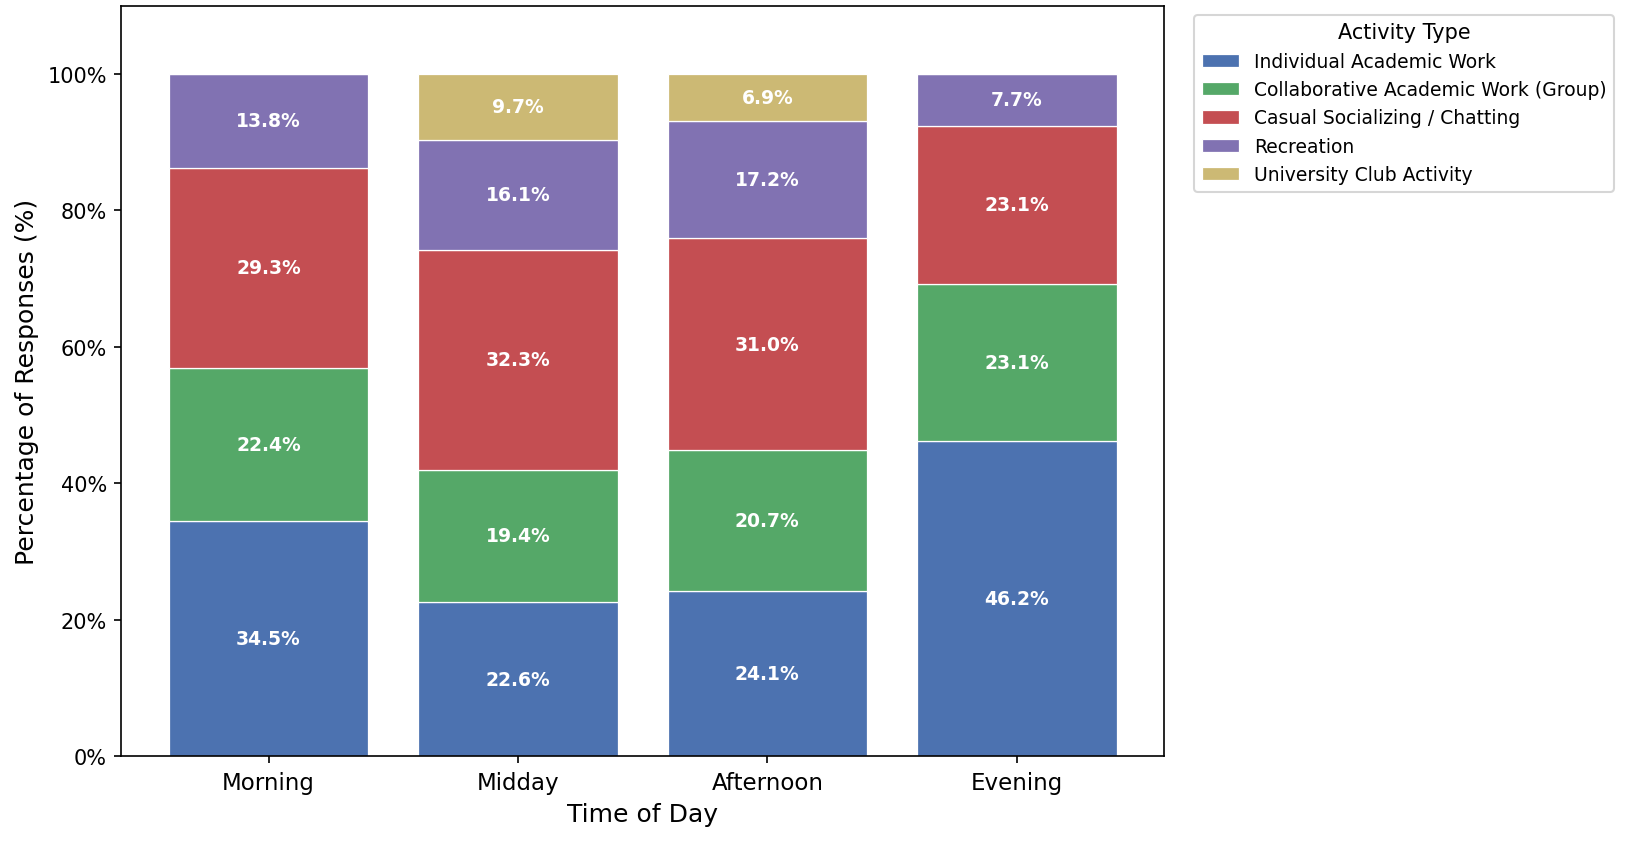
\includegraphics[width=0.7\linewidth]{interval_vs_activity.png}
    \caption{Activities performed in the Open area by time of day}
    \label{fig:Activities}
\end{figure}
The figure indicates that the usage of the Open Area fluctuates during the different times of the day. The periods of Morning and Evening are occupied predominantly with Individual Academic Activity, due to the reason that they are characterized by less occupancy and favorable conditions for studying. Midday and Afternoon periods accommodate both academic and social activities, since there is an increase in the occupancy at those times. The afternoon period has the highest percentage of Collaborative Academic Activity, which makes it the favorite period for discussion among students. Although the environmental conditions at the Evening period are favorable, the low use of it can be attributed to various factors including poor lighting.


\section{Environmental effects}
The line graph depicts the average ratings of the four factors: Thermal Comfort, Noise Level, Occupancy Level, and Weather Conditions in relation to the four periods during the day. In general, it can be noted that the environmental conditions deteriorate throughout the day, especially comparing the Morning and Midday periods. The lowest average ratings of Thermal Comfort (1.55), Noise Level (1.34), and Weather Conditions (2.10) are obtained at Midday; this is also the period when occupancy achieves its highest rating (4.86), which makes it the least comfortable period during the day. The conditions start improving during the Afternoon period because the occupancy levels decrease. At Evening, Thermal Comfort (4.42), Noise Level (4.27), and Weather Conditions (4.31) receive the highest ratings along with the lowest occupancy level (1.65).(these fields are rated in the survey as, (1 = Very Disruptive, 5 = Excellent/Perfect))

\begin{figure}[H] 
    \centering
    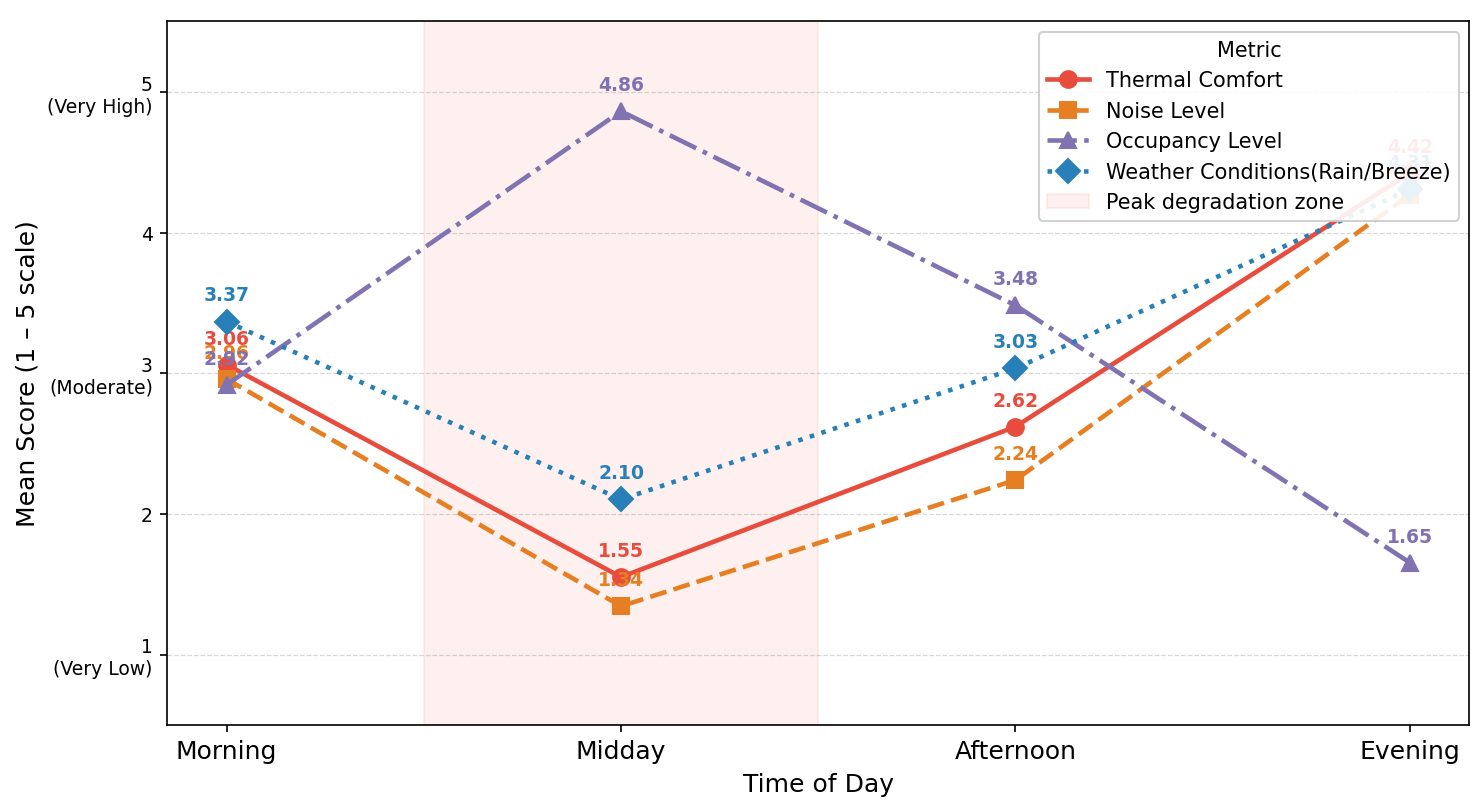
\includegraphics[width=0.7\linewidth]{trend_a_diurnal_degradation.png}
    \caption{Environmental effects}
    \label{fig:Env}
\end{figure}

When these environmental trends are compared with the observed activity patterns, a clear relationship between environmental conditions and student behavior becomes apparent. During the Morning, moderate comfort levels and relatively low occupancy are accompanied by the highest proportion of Individual Academic Work. As environmental conditions become less comfortable and occupancy reaches its peak during Midday, the proportion of Casual Socializing and Recreational activities increases, suggesting that less favorable conditions reduce students' tendency to engage in focused individual study. As conditions improve in the Afternoon, Collaborative Academic Work becomes more common, while the comfortable environment and lower occupancy observed during the Evening are associated with a return to Individual Academic Work as the dominant activity. Overall, these findings indicate that students' use of the Open Area for academic purposes is closely related to the quality of the surrounding environment, with the space naturally shifting between periods of individual study, collaborative work, and social interaction throughout the day.

\section{Infrastructure needs}
\begin{figure}[H] 
    \centering
    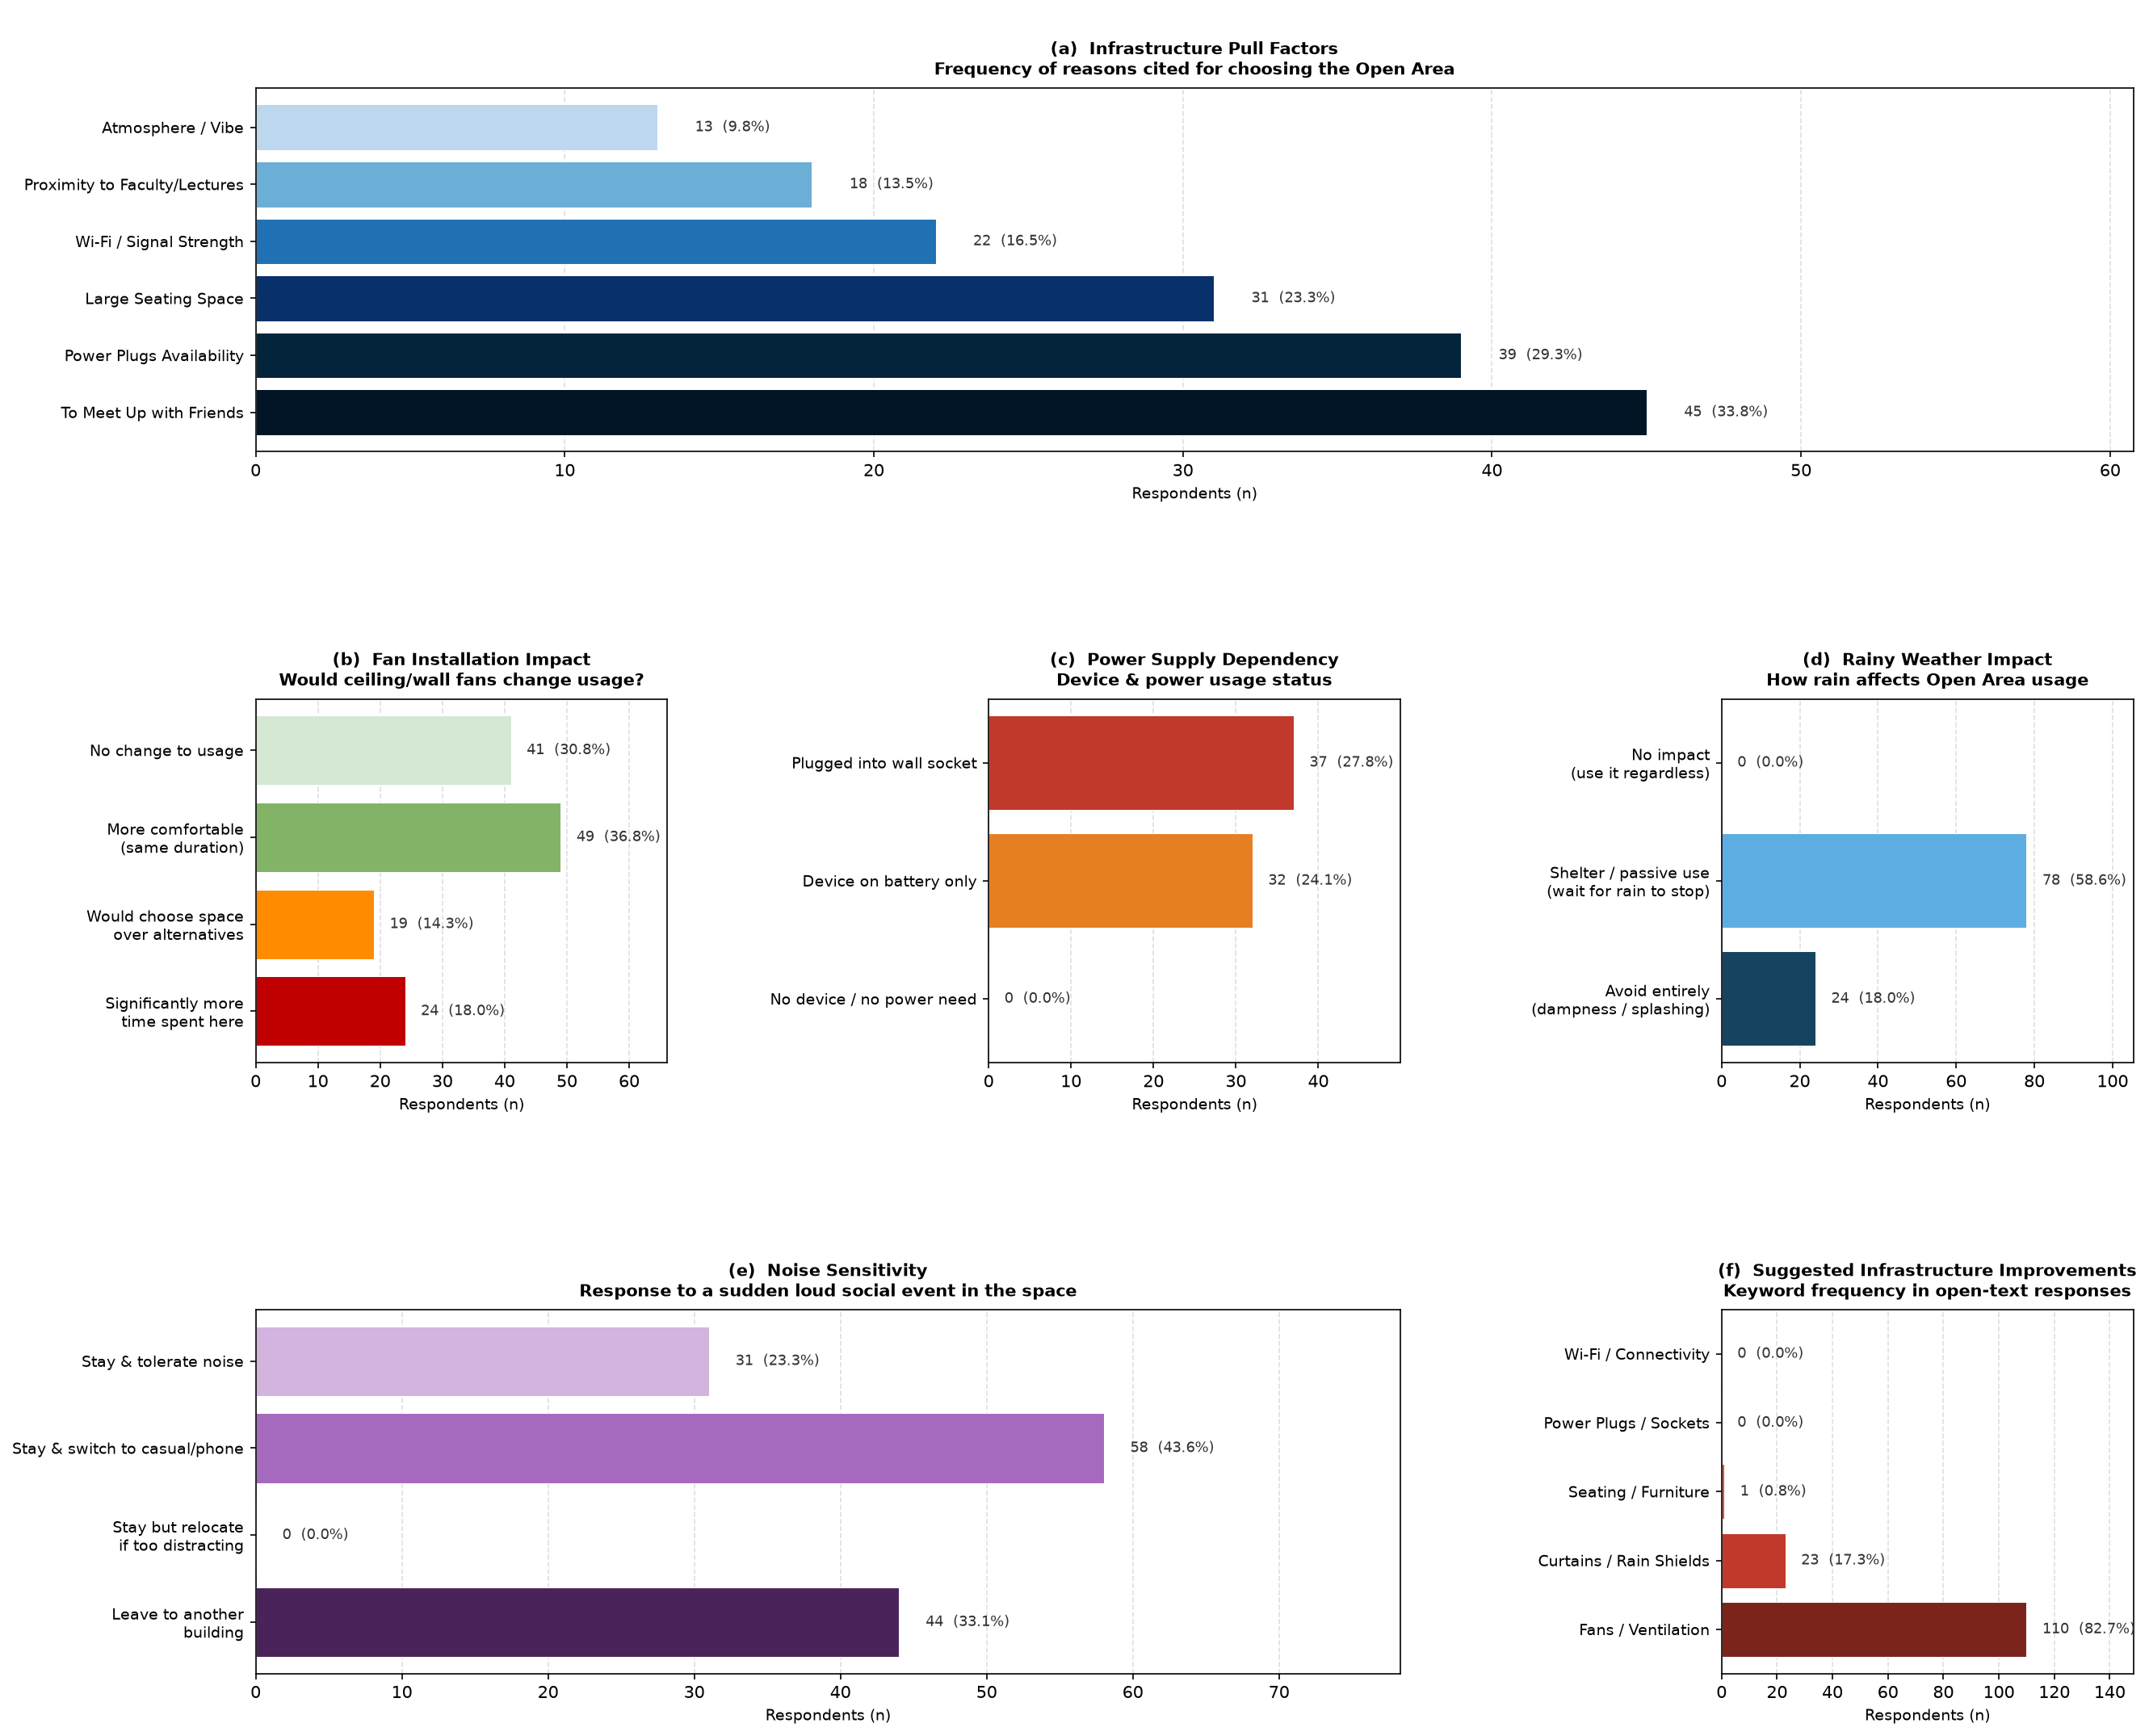
\includegraphics[width=0.9\linewidth]{infrastructure_analysis.png}
    \caption{Infrastructure analysis}
    \label{fig:Infrastructure}
\end{figure}

\textbf{(a) Infrastructure Pull Factors}

Panel (a) reveals that the decision to utilize the Open Area is based not only on social factors but also on the associated infrastructure. Power outlet and Wi-Fi are some of the key factors driving usage, which means that many students depend on this infrastructure for using their electronic devices during learning. Together with panel (c), this demonstrates the role of robust infrastructure in attracting users.

\vspace{0.5cm}

\textbf{(b) Effectiveness of Fan Installation}

Panel (b) implies that fan installation will help improve both comfort level and academic usage of the Open Area. Many participants revealed that they would spend more time in studying and even pick the Open Area over other places if fans were installed here.

\vspace{0.5cm}

\textbf{(c) Power Supply Dependence}

Panel (c) proves that access to electricity is important for many users since over half of the respondents use electric appliances. Together with faulty sockets, this information means that the infrastructure of electricity determines the duration of study sessions in the Open Area.

\textbf{(d) Effect of Rainy Weather on Usage}

The results presented in panel (d) indicate that rain adversely affects the use of the Open Area for educational purposes, with majority of the students preferring the area as a place of shelter or not using the area at all.

\vspace{0.5cm}

\textbf{(e) Effect of Noise}

As seen in panel (e), noise greatly affects the ability of students to conduct studies within the Open Area, as most respondents will be forced to either pause their studying or leave the area when there is noise going on.

\vspace{0.5cm}

\textbf{(f) Suggested Infrastructure Improvements}

Panel (f) provides a clear, student-defined priority order that is consistent with every other finding in this section. The near-unanimous call for fans directly corresponds to the thermal collapse identified in the diurnal curve and the behavioral shift away from academic work at Midday. The secondary demand for curtains and rain shields addresses the weather vulnerability that strips the space of academic utility during rainfall. What is equally telling is what respondents did not mention prominently: seating, Wi-Fi, and power plugs feature minimally in open-text suggestions, not because they are unimportant --- Panel (a) and (c) confirm they are --- but because students appear to frame the plug and connectivity problems as maintenance failures rather than missing infrastructure, and therefore do not articulate them as new investments. The convergence of the quantitative and qualitative signals in this panel points to a clear and actionable infrastructure priority: address thermal comfort first through fan installation, then weather protection, with maintenance of existing electrical and connectivity infrastructure as an ongoing obligation.
\vspace{0.5cm}

\chapter{Critical Analysis}
The quantitative results affirm various observations made during the qualitative study and reveal that the purpose of the UCSC Open Area varies according to the time of day and environmental factors as opposed to being just a study space.

According to the survey, the main users of the Open Area are the students of UCSC, especially first- and second-year undergraduate students, while the students from other departments utilize the space relatively rarely. The usage pattern also differs during the day: the mornings and evenings are characterized by mostly academic work as a result of low occupation and good environmental factors, while collaborative activities and socializing become more frequent during the middle of the day and late afternoon.

The infrastructure becomes very important in maintaining academic utility. While most students come to socialize, infrastructural facilities like power sockets, seating arrangements, and connectivity promote long durations of stay at the place. It becomes evident that the high requirement for fans, along with the effect of noise and rainy weather, makes thermal comfort and environmental protection the top two factors needing improvement.

In general, the research findings show that the performance of the Open Area depends on the interplay between academic considerations, social considerations, environmental comfort, and infrastructure facilities.

\chapter{Conclusion and Future Work}

\section{Conclusion}

The quantitative stage of this study was able to validate and further build upon the conclusions reached through the previous qualitative stage as it involved collecting quantifiable data from a greater number of students. The data collected through surveys and structured observation has revealed a better insight into the nature of students' activities in UCSC Open Area and has helped to uncover the factors that impact their choice of the place.

It can be seen that there are differences in students' activities depending on environmental factors such as occupancy level, thermal comfort, weather, and noise. Moreover, the availability of infrastructures like power outlets, seating space, and ventilation also impacts positively on the students' ability to carry out academic work in the Open Area.

In general, this stage converted the qualitative information collected through the qualitative study into credible quantitative data. These results lay a firm basis for the next step in research, which will involve the integration of both qualitative and quantitative results into final conclusions and recommendations concerning the UCSC Open Area.

\section{Future Work}
In the final stage of the study, statistical tools shall be used to test for usage patterns and their environmental implications in the open space. The Chi-Square Test, Mann-Whitney U Test, and Kruskal-Wallis Test shall be used to investigate associations between usage times of day, types of activities, school year and environmental comfort.

In order to ensure robustness of findings, responses in the surveys would be triangulated with observed data by testing the relationship between perceived and actual occupant counts and perceived and actual environmental levels by using the Spearman’s Rank Correlation method.

After that, a Binary Logistic Regression Model would be constructed to predict the probability of students leaving the open space given different environmental factors like noise, thermal comfort and availability of electricity. It would provide information about factors causing student displacement.

Finally, findings of statistical analysis will provide scientific justification for recommendations for UCSC, such as spatial zones for activities, installation of fans and rain shelters.

\begin{center}
    * * * * *
\end{center}

\printindex

\end{document}